\documentclass{standalone}
\usepackage{tikz}
\usetikzlibrary{patterns, positioning}
\usepackage[sfdefault]{ClearSans} %% option 'sfdefault' activates Clear Sans as the default text font
\usepackage[T1]{fontenc}

\begin{document}
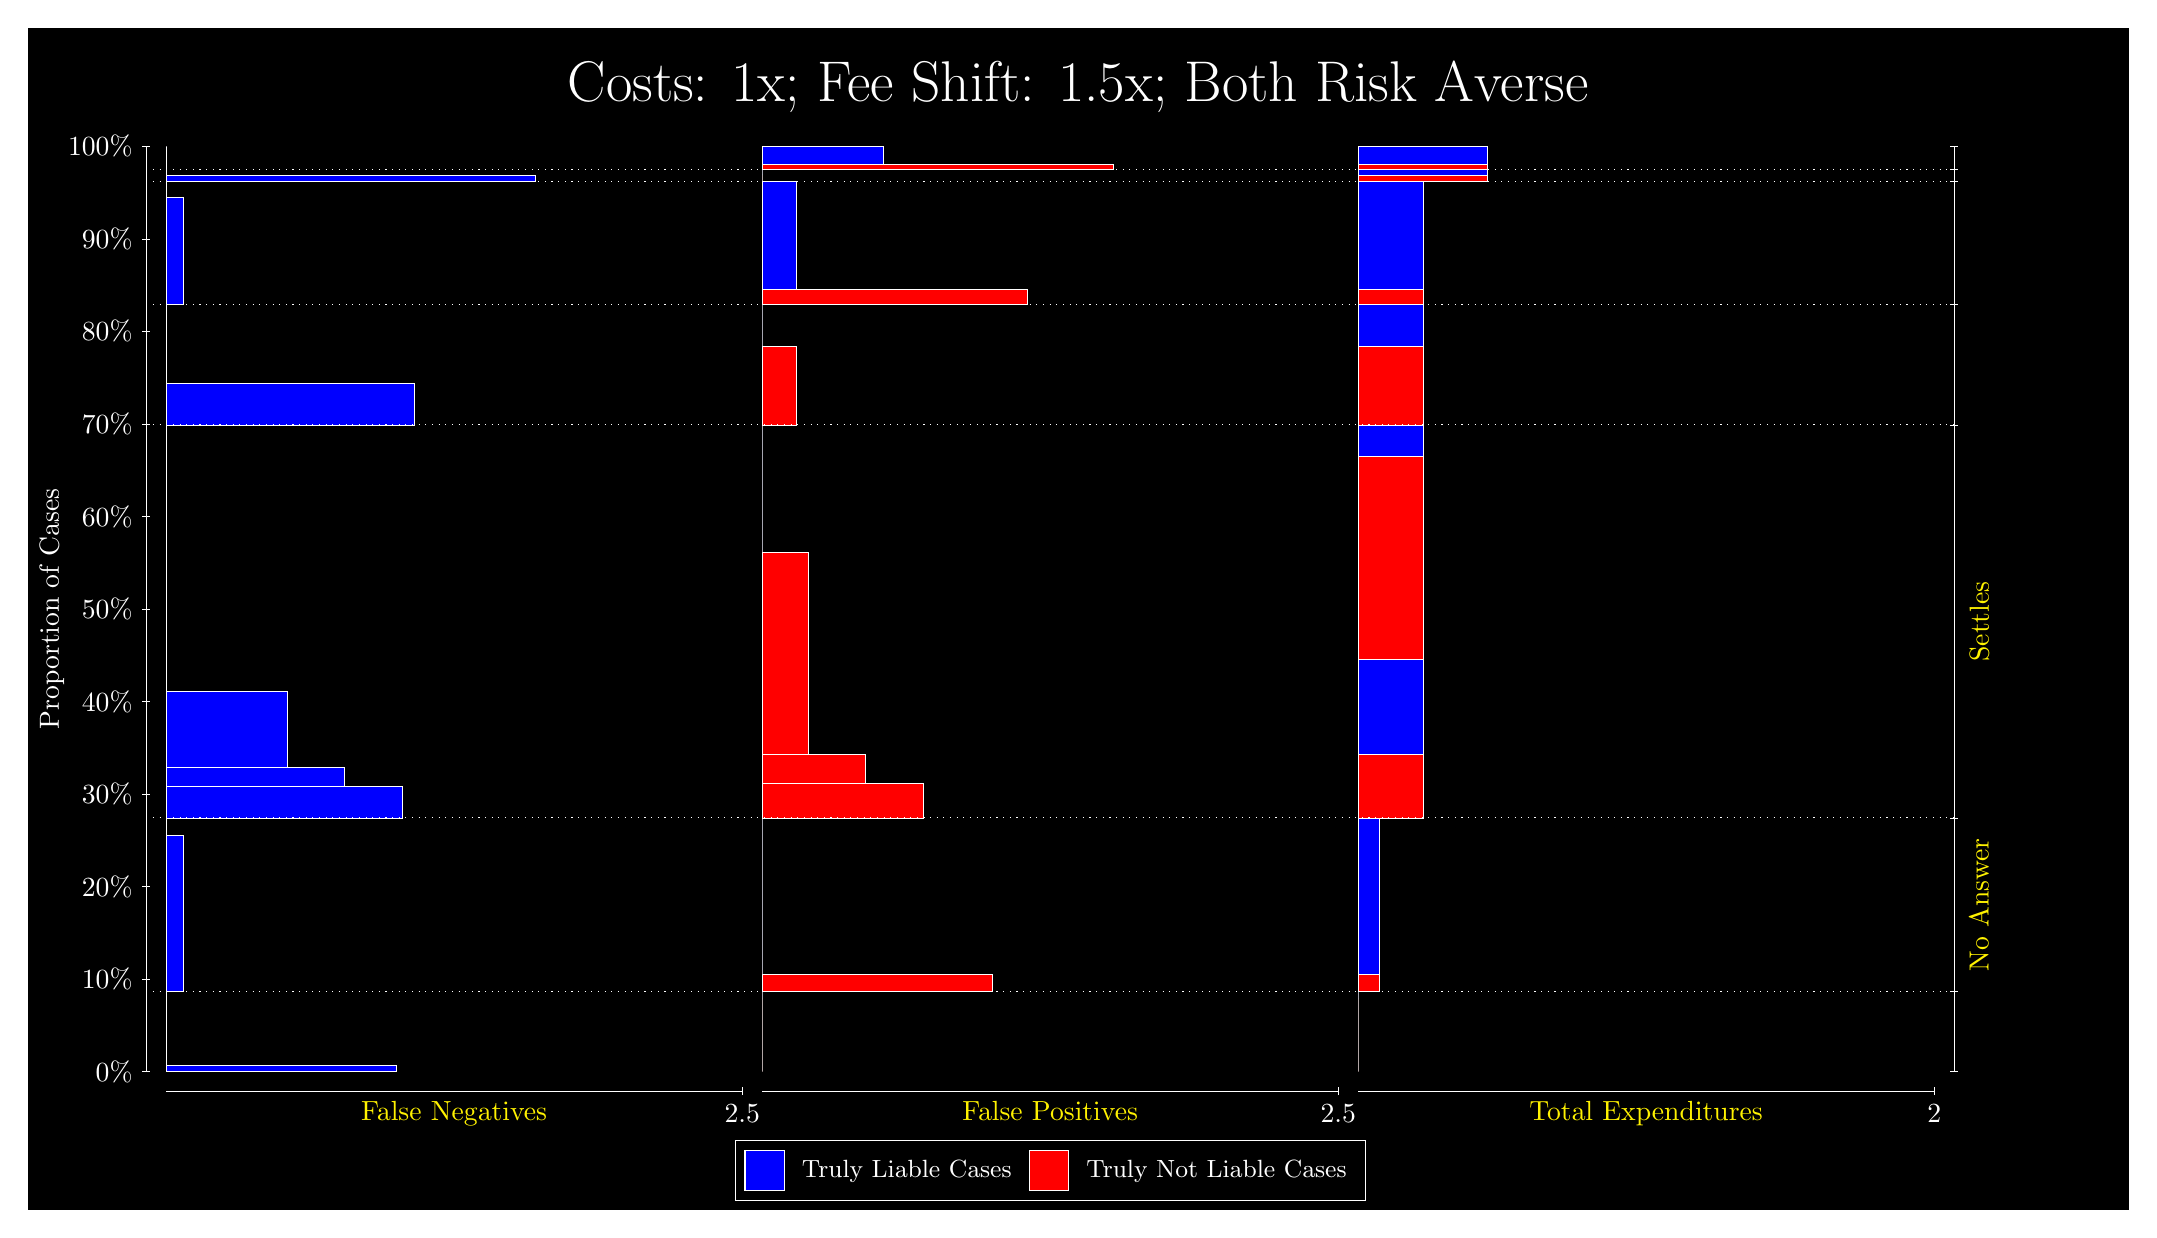
\begin{tikzpicture}
\draw[fill=black] (0,0) rectangle (26.667,15);
\draw[text=white] (0,13.5) rectangle (26.667,15) node[midway] {\huge Costs: 1x; Fee Shift: 1.5x; Both Risk Averse};
\draw[white, very thin] (1.5,1.75) -- (1.5,13.5);
\node[rotate=90, text=white, anchor=center] at (0.3, 7.625) {Proportion of Cases};
\draw[white, very thin] (1.45,1.75) -- (1.55,1.75);
\node[text=white, anchor=east] at (1.45, 1.75) {0\%};
\draw[white, very thin] (1.45,2.925) -- (1.55,2.925);
\node[text=white, anchor=east] at (1.45, 2.925) {10\%};
\draw[white, very thin] (1.45,4.1) -- (1.55,4.1);
\node[text=white, anchor=east] at (1.45, 4.1) {20\%};
\draw[white, very thin] (1.45,5.275) -- (1.55,5.275);
\node[text=white, anchor=east] at (1.45, 5.275) {30\%};
\draw[white, very thin] (1.45,6.45) -- (1.55,6.45);
\node[text=white, anchor=east] at (1.45, 6.45) {40\%};
\draw[white, very thin] (1.45,7.625) -- (1.55,7.625);
\node[text=white, anchor=east] at (1.45, 7.625) {50\%};
\draw[white, very thin] (1.45,8.8) -- (1.55,8.8);
\node[text=white, anchor=east] at (1.45, 8.8) {60\%};
\draw[white, very thin] (1.45,9.975) -- (1.55,9.975);
\node[text=white, anchor=east] at (1.45, 9.975) {70\%};
\draw[white, very thin] (1.45,11.15) -- (1.55,11.15);
\node[text=white, anchor=east] at (1.45, 11.15) {80\%};
\draw[white, very thin] (1.45,12.325) -- (1.55,12.325);
\node[text=white, anchor=east] at (1.45, 12.325) {90\%};
\draw[white, very thin] (1.45,13.5) -- (1.55,13.5);
\node[text=white, anchor=east] at (1.45, 13.5) {100\%};

\draw[white, very thin] (24.457,1.75) -- (24.457,13.5);
\draw[white, very thin] (24.407,1.75) -- (24.507,1.75);
\node[anchor=west] at (24.407, 1.75) {};
\draw[white, very thin] (24.407,2.7636) -- (24.507,2.7636);
\node[anchor=west] at (24.407, 2.7636) {};
\draw[white, very thin] (24.407,4.9714) -- (24.507,4.9714);
\node[anchor=west] at (24.407, 4.9714) {};
\draw[white, very thin] (24.407,9.9617) -- (24.507,9.9617);
\node[anchor=west] at (24.407, 9.9617) {};
\draw[white, very thin] (24.407,11.488) -- (24.507,11.488);
\node[anchor=west] at (24.407, 11.488) {};
\draw[white, very thin] (24.407,13.058) -- (24.507,13.058);
\node[anchor=west] at (24.407, 13.058) {};
\draw[white, very thin] (24.407,13.207) -- (24.507,13.207);
\node[anchor=west] at (24.407, 13.207) {};
\draw[white, very thin] (24.407,13.5) -- (24.507,13.5);
\node[anchor=west] at (24.407, 13.5) {};

\draw[white, very thin, fill=blue] (1.75,1.75) rectangle (4.6775,1.832);
\draw[white, very thin, fill=red] (1.75,1.832) rectangle (1.75,2.7636);
\draw[white, very thin, fill=blue] (1.75,2.7636) rectangle (1.9696,4.7518);
\draw[white, very thin, fill=red] (1.75,4.7518) rectangle (1.75,4.9714);
\draw[white, very thin, fill=blue] (1.75,4.9714) rectangle (4.7507,5.369);
\draw[white, very thin, fill=blue] (1.75,5.369) rectangle (4.0188,5.6128);
\draw[white, very thin, fill=blue] (1.75,5.6128) rectangle (3.287,6.5842);
\draw[white, very thin, fill=red] (1.75,6.5842) rectangle (1.75,9.9617);
\draw[white, very thin, fill=blue] (1.75,9.9617) rectangle (4.8971,10.492);
\draw[white, very thin, fill=red] (1.75,10.492) rectangle (1.75,11.488);
\draw[white, very thin, fill=blue] (1.75,11.488) rectangle (1.9696,12.856);
\draw[white, very thin, fill=red] (1.75,12.856) rectangle (1.75,13.058);
\draw[white, very thin, fill=blue] (1.75,13.058) rectangle (6.4341,13.129);
\draw[white, very thin, fill=red] (1.75,13.129) rectangle (1.75,13.207);
\draw[white, very thin, fill=red] (1.75,13.207) rectangle (1.75,13.278);
\draw[white, very thin, fill=blue] (1.75,13.278) rectangle (1.75,13.5);
\draw[white, very thin, fill=red] (9.3189,1.75) rectangle (9.3189,2.6815);
\draw[white, very thin, fill=blue] (9.3189,2.6815) rectangle (9.3189,2.7636);
\draw[white, very thin, fill=red] (9.3189,2.7636) rectangle (12.246,2.9832);
\draw[white, very thin, fill=blue] (9.3189,2.9832) rectangle (9.3189,4.9714);
\draw[white, very thin, fill=red] (9.3189,4.9714) rectangle (11.368,5.4092);
\draw[white, very thin, fill=red] (9.3189,5.4092) rectangle (10.636,5.7729);
\draw[white, very thin, fill=red] (9.3189,5.7729) rectangle (9.9044,8.3489);
\draw[white, very thin, fill=blue] (9.3189,8.3489) rectangle (9.3189,9.9617);
\draw[white, very thin, fill=red] (9.3189,9.9617) rectangle (9.758,10.957);
\draw[white, very thin, fill=blue] (9.3189,10.957) rectangle (9.3189,11.488);
\draw[white, very thin, fill=red] (9.3189,11.488) rectangle (12.686,11.69);
\draw[white, very thin, fill=blue] (9.3189,11.69) rectangle (9.758,13.058);
\draw[white, very thin, fill=red] (9.3189,13.058) rectangle (9.3189,13.136);
\draw[white, very thin, fill=blue] (9.3189,13.136) rectangle (9.3189,13.207);
\draw[white, very thin, fill=red] (9.3189,13.207) rectangle (13.783,13.278);
\draw[white, very thin, fill=blue] (9.3189,13.278) rectangle (10.856,13.5);
\draw[white, very thin, fill=red] (16.888,1.75) rectangle (16.888,2.6815);
\draw[white, very thin, fill=blue] (16.888,2.6815) rectangle (16.888,2.7636);
\draw[white, very thin, fill=red] (16.888,2.7636) rectangle (17.162,2.9832);
\draw[white, very thin, fill=blue] (16.888,2.9832) rectangle (17.162,4.9714);
\draw[white, very thin, fill=red] (16.888,4.9714) rectangle (17.711,5.7729);
\draw[white, very thin, fill=blue] (16.888,5.7729) rectangle (17.711,6.9881);
\draw[white, very thin, fill=red] (16.888,6.9881) rectangle (17.711,9.5641);
\draw[white, very thin, fill=blue] (16.888,9.5641) rectangle (17.711,9.9617);
\draw[white, very thin, fill=red] (16.888,9.9617) rectangle (17.711,10.957);
\draw[white, very thin, fill=blue] (16.888,10.957) rectangle (17.711,11.488);
\draw[white, very thin, fill=red] (16.888,11.488) rectangle (17.711,11.69);
\draw[white, very thin, fill=blue] (16.888,11.69) rectangle (17.711,13.058);
\draw[white, very thin, fill=red] (16.888,13.058) rectangle (18.534,13.136);
\draw[white, very thin, fill=blue] (16.888,13.136) rectangle (18.534,13.207);
\draw[white, very thin, fill=red] (16.888,13.207) rectangle (18.534,13.278);
\draw[white, very thin, fill=blue] (16.888,13.278) rectangle (18.534,13.5);
\draw[white, dotted] (1.5,2.7636) -- (24.457,2.7636);
\draw[white, dotted] (1.5,4.9714) -- (24.457,4.9714);
\draw[white, dotted] (1.5,9.9617) -- (24.457,9.9617);
\draw[white, dotted] (1.5,11.488) -- (24.457,11.488);
\draw[white, dotted] (1.5,13.058) -- (24.457,13.058);
\draw[white, dotted] (1.5,13.207) -- (24.457,13.207);
\draw[white, very thin] (1.75,1.5) -- (9.0689,1.5);
\node[text=yellow, anchor=north] at (5.4094, 1.5) {False Negatives};
\draw[white, very thin] (9.0689,1.45) -- (9.0689,1.55);
\node[text=white, anchor=north] at (9.0689, 1.45) {2.5};

\draw[white, very thin] (9.3189,1.5) -- (16.638,1.5);
\node[text=yellow, anchor=north] at (12.978, 1.5) {False Positives};
\draw[white, very thin] (16.638,1.45) -- (16.638,1.55);
\node[text=white, anchor=north] at (16.638, 1.45) {2.5};

\draw[white, very thin] (16.888,1.5) -- (24.207,1.5);
\node[text=yellow, anchor=north] at (20.547, 1.5) {Total Expenditures};
\draw[white, very thin] (24.207,1.45) -- (24.207,1.55);
\node[text=white, anchor=north] at (24.207, 1.45) {2};


\node[text=yellow, centered, rotate=90] at (24.777, 3.8675) {No Answer};
\node[text=yellow, centered, rotate=90] at (24.777, 7.4665) {Settles};





\draw (12.978300999999998,1.5) node[draw=none] (baseCoordinate) {};
\begin{scope}[align=center]
        \matrix[scale=0.5, draw=white, below=0.5cm of baseCoordinate, nodes={draw}, column sep=0.1cm]{
            \node[rectangle, draw, minimum width=0.5cm, minimum height=0.5cm, fill=blue] {}; &
            \node[draw=none, font=\small, text=white] (B) {Truly Liable Cases}; &
            \node[rectangle, draw, minimum width=0.5cm, minimum height=0.5cm, fill=red] {}; &
            \node[draw=none, font=\small, text=white] (B) {Truly Not Liable Cases}; \\
            };
\end{scope}

\end{tikzpicture}
\end{document}